\documentclass[12pt,a4paper]{article}
\usepackage[UTF8]{ctex}
\usepackage{amsmath}
\usepackage{amssymb}
\usepackage{amsthm}
\usepackage{graphicx}
\usepackage{hyperref}
\usepackage{geometry}
\usepackage{listings}
\usepackage{xcolor}
\usepackage{fancyhdr}
\geometry{left=2cm,right=2cm,top=2.5cm,bottom=2.5cm,headheight=15pt}
\setlength{\baselineskip}{1.1\baselineskip}
\setlength{\parskip}{0.5em}

% 导入通用样式
% 通用样式文件 - 统一所有文档的样式

% 目录样式设置 - 干净简洁,无边框,优化编号
% 使用基本 LaTeX 命令美化目录
\makeatletter
\renewcommand\@dotsep{2}
% 优化编号格式:减少缩进,使编号更紧凑
\renewcommand\l@section{\@dottedtocline{1}{0em}{1.2em}}
\renewcommand\l@subsection{\@dottedtocline{2}{1.2em}{1.8em}}
\renewcommand\l@subsubsection{\@dottedtocline{3}{3em}{2.2em}}
% 设置目录深度为3,显示到subsubsection级别
\setcounter{tocdepth}{3}
\makeatother

% 超链接设置 - 目录链接无颜色框
\hypersetup{
    colorlinks=true,
    linkcolor=black,          % 目录链接为黑色
    filecolor=black,
    urlcolor=blue,
    citecolor=black,
    pdfstartview=FitH,
    pdfborder={0 0 0},        % 无边框
    linkbordercolor={0 0 0},  % 链接边框颜色为黑色(不可见)
    pdfborderstyle={/S/U},    % 无边框样式
}

% 页眉页脚设置(在文档中重新定义)
\usepackage{fancyhdr}
% 注意:每个文档需要在导入 common_style.tex 后设置自己的页眉页脚

% 章节格式 - 简洁美观(使用基本命令)
\makeatletter
\renewcommand\section{\@startsection {section}{1}{\z@}%
                                   {-3.5ex \@plus -1ex \@minus -.2ex}%
                                   {2.3ex \@plus.2ex}%
                                   {\normalfont\Large\bfseries}}
\renewcommand\subsection{\@startsection{subsection}{2}{\z@}%
                                     {-3.25ex\@plus -1ex \@minus -.2ex}%
                                     {1.5ex \@plus .2ex}%
                                     {\normalfont\large\bfseries}}
\renewcommand\subsubsection{\@startsection{subsubsection}{3}{\z@}%
                                     {-3.25ex\@plus -1ex \@minus -.2ex}%
                                     {1.5ex \@plus .2ex}%
                                     {\normalfont\normalsize\bfseries}}
\makeatother

% 代码样式设置 - 简洁干净,无背景色
\definecolor{codegray}{rgb}{0.5,0.5,0.5}
\definecolor{keywordblue}{rgb}{0,0,0.8}
\definecolor{stringred}{rgb}{0.3,0.3,0.3}
\definecolor{commentgreen}{rgb}{0,0.5,0}

\lstdefinestyle{pythonstyle}{
    language=Python,
    % 无背景色 - 使用白色背景,与文档背景一致
    commentstyle=\color{commentgreen},      % 注释不用斜体
    keywordstyle=\color{keywordblue}\bfseries,
    stringstyle=\color{stringred},
    basicstyle=\ttfamily\small,
    breakatwhitespace=false,
    breaklines=true,
    captionpos=b,
    keepspaces=true,
    numbers=none,                           % 不显示行号
    showspaces=false,
    showstringspaces=false,
    showtabs=false,
    tabsize=4,
    frame=single,                          % 保留边框,但更简洁
    rulecolor=\color{black},
    framerule=0.5pt,                       % 细边框
    framexleftmargin=8pt,                  % 左边距(代码与左边框的距离)
    framexrightmargin=8pt,                 % 右边距(代码与右边框的距离)
    framextopmargin=6pt,                   % 上边距(代码与上边框的距离)
    framexbottommargin=6pt,                % 下边距(代码与下边框的距离)
    morekeywords={import,from,as,class,def,return,yield,lambda,if,elif,else,for,while,break,continue,pass,try,except,finally,raise,assert,with,del,global,nonlocal,and,or,not,in,is},
    identifierstyle=\color{black},
}

\lstset{style=pythonstyle}

% 封面宏定义
\newcommand{\makecover}[5]{%
    \newpage
    \thispagestyle{empty}
    \vspace*{1.5cm}
    \begin{center}
        \vspace{2cm}
        {\fontsize{48}{58}\selectfont\bfseries #1}\\[0.8cm]
        \vspace{1.5cm}
        {\Large #2}\\[0.4cm]
        \vspace{1.5cm}
        {\large #3}\\[1.5cm]
        
        % 神经网络图 - 紧凑版本,无标签
        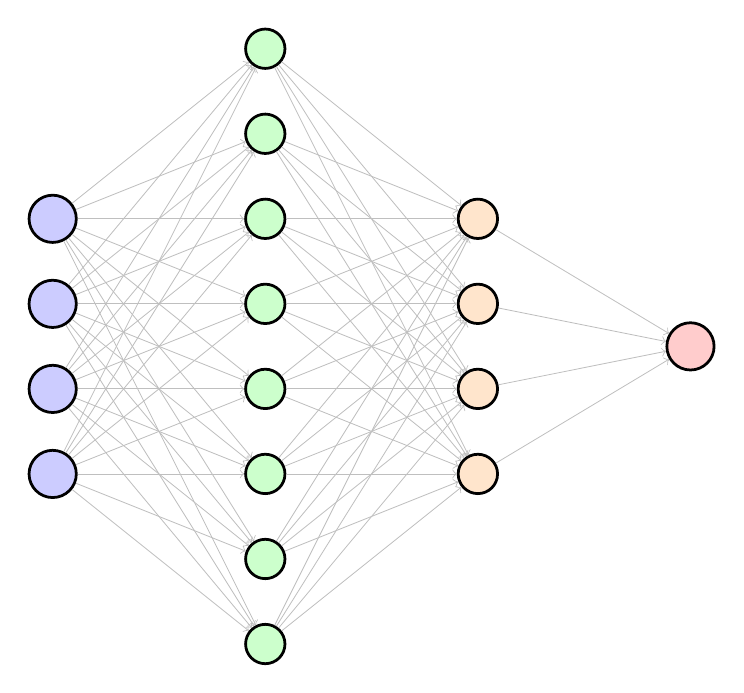
\begin{tikzpicture}[scale=0.9]
        % 定义神经元间距
        \def\spacing{1.2}
        
        % 输入层 - 4个神经元,关于横轴对称
        \node[circle, draw, minimum size=0.6cm, fill=blue!20, line width=1pt] (x1) at (0, -1.8) {};
        \node[circle, draw, minimum size=0.6cm, fill=blue!20, line width=1pt] (x2) at (0, -0.6) {};
        \node[circle, draw, minimum size=0.6cm, fill=blue!20, line width=1pt] (x3) at (0, 0.6) {};
        \node[circle, draw, minimum size=0.6cm, fill=blue!20, line width=1pt] (x4) at (0, 1.8) {};
        
        % 隐藏层1 - 8个神经元,关于横轴对称
        \node[circle, draw, minimum size=0.5cm, fill=green!20, line width=1pt] (h11) at (3, -4.2) {};
        \node[circle, draw, minimum size=0.5cm, fill=green!20, line width=1pt] (h12) at (3, -3.0) {};
        \node[circle, draw, minimum size=0.5cm, fill=green!20, line width=1pt] (h13) at (3, -1.8) {};
        \node[circle, draw, minimum size=0.5cm, fill=green!20, line width=1pt] (h14) at (3, -0.6) {};
        \node[circle, draw, minimum size=0.5cm, fill=green!20, line width=1pt] (h15) at (3, 0.6) {};
        \node[circle, draw, minimum size=0.5cm, fill=green!20, line width=1pt] (h16) at (3, 1.8) {};
        \node[circle, draw, minimum size=0.5cm, fill=green!20, line width=1pt] (h17) at (3, 3.0) {};
        \node[circle, draw, minimum size=0.5cm, fill=green!20, line width=1pt] (h18) at (3, 4.2) {};
        
        % 隐藏层2 - 4个神经元,关于横轴对称
        \node[circle, draw, minimum size=0.5cm, fill=orange!20, line width=1pt] (h21) at (6, -1.8) {};
        \node[circle, draw, minimum size=0.5cm, fill=orange!20, line width=1pt] (h22) at (6, -0.6) {};
        \node[circle, draw, minimum size=0.5cm, fill=orange!20, line width=1pt] (h23) at (6, 0.6) {};
        \node[circle, draw, minimum size=0.5cm, fill=orange!20, line width=1pt] (h24) at (6, 1.8) {};
        
        % 输出层 - 1个神经元,在横轴上
        \node[circle, draw, minimum size=0.6cm, fill=red!20, line width=1pt] (y) at (9, 0) {};
        
        % 输入层到隐藏层1的连接
        \foreach \i in {1,...,4}
            \foreach \j in {1,...,8}
                \draw[->, gray!50, line width=0.3pt] (x\i) -- (h1\j);
        
        % 隐藏层1到隐藏层2的连接
        \foreach \i in {1,...,8}
            \foreach \j in {1,...,4}
                \draw[->, gray!50, line width=0.3pt] (h1\i) -- (h2\j);
        
        % 隐藏层2到输出层的连接
        \foreach \i in {1,...,4}
            \draw[->, gray!50, line width=0.3pt] (h2\i) -- (y);
        \end{tikzpicture}
        
        \vfill
        \vspace{2cm}
        {\normalsize #5}
        \vspace{1.5cm}
    \end{center}
    \newpage
}



% 页眉页脚设置
\pagestyle{fancy}
\fancyhf{}
\fancyhead[L]{\leftmark}
\fancyhead[R]{\thepage}
\fancyfoot[C]{\small AI/ML 综合练习题答案}
\renewcommand{\headrulewidth}{0.3pt}
\renewcommand{\footrulewidth}{0.3pt}

\title{AI/ML 综合练习题答案}
\author{}
\date{\today}

\newtheorem{definition}{定义}[section]
\newtheorem{example}{例}[section]

\begin{document}

% 封面
\makecover{AI/ML 综合练习题答案}{数学基础 · 深度学习 · 大语言模型 · Python 编程}{详细解答与代码实现}{AI/ML 系列教程}

\maketitle

\tableofcontents
\newpage

\part{数学基础练习题答案}

\section{计算题答案}

\subsection{矩阵运算}

\begin{enumerate}
    \item \textbf{矩阵乘法}:
    \begin{align}
    \mathbf{A}\mathbf{B} &= \begin{bmatrix} 1 & 2 \\ 3 & 4 \end{bmatrix} \begin{bmatrix} 5 & 6 \\ 7 & 8 \end{bmatrix} \\
    &= \begin{bmatrix} 1 \times 5 + 2 \times 7 & 1 \times 6 + 2 \times 8 \\ 3 \times 5 + 4 \times 7 & 3 \times 6 + 4 \times 8 \end{bmatrix} \\
    &= \begin{bmatrix} 19 & 22 \\ 43 & 50 \end{bmatrix}
    \end{align}
    
    \textbf{转置}:
    \begin{equation}
    \mathbf{A}^T = \begin{bmatrix} 1 & 3 \\ 2 & 4 \end{bmatrix}
    \end{equation}
    
    \textbf{逆矩阵}:
    \begin{align}
    \det(\mathbf{A}) &= 1 \times 4 - 2 \times 3 = -2 \\
    \mathbf{A}^{-1} &= \frac{1}{-2} \begin{bmatrix} 4 & -2 \\ -3 & 1 \end{bmatrix} = \begin{bmatrix} -2 & 1 \\ 1.5 & -0.5 \end{bmatrix}
    \end{align}
    
    \item \textbf{向量范数}:
    \begin{align}
    \|\mathbf{x}\|_1 &= |1| + |2| + |3| = 6 \\
    \|\mathbf{x}\|_2 &= \sqrt{1^2 + 2^2 + 3^2} = \sqrt{14} \approx 3.74 \\
    \|\mathbf{x}\|_\infty &= \max(|1|, |2|, |3|) = 3
    \end{align}
    
    \item \textbf{点积和余弦相似度}:
    \begin{align}
    \mathbf{u} \cdot \mathbf{v} &= 1 \times 0 + 0 \times 1 + 1 \times 1 = 1 \\
    \|\mathbf{u}\|_2 &= \sqrt{1^2 + 0^2 + 1^2} = \sqrt{2} \\
    \|\mathbf{v}\|_2 &= \sqrt{0^2 + 1^2 + 1^2} = \sqrt{2} \\
    \cos(\theta) &= \frac{\mathbf{u} \cdot \mathbf{v}}{\|\mathbf{u}\|_2 \|\mathbf{v}\|_2} = \frac{1}{\sqrt{2} \times \sqrt{2}} = \frac{1}{2}
    \end{align}
\end{enumerate}

\subsection{概率计算}

\begin{enumerate}
    \item \textbf{二项分布}:
    \begin{align}
    P(X = 2) &= \binom{3}{2} \left(\frac{1}{2}\right)^2 \left(\frac{1}{2}\right)^{3-2} \\
    &= 3 \times \frac{1}{4} \times \frac{1}{2} = \frac{3}{8} = 0.375
    \end{align}
    
    \item \textbf{标准正态分布}:
    \begin{align}
    P(-1 < X < 1) &= \Phi(1) - \Phi(-1) \\
    &= \Phi(1) - (1 - \Phi(1)) \\
    &= 2\Phi(1) - 1 \\
    &\approx 2 \times 0.8413 - 1 = 0.6826
    \end{align}
    其中 $\Phi$ 是标准正态分布的累积分布函数。
    
    \item \textbf{贝叶斯定理}:
    \begin{align}
    P(A|B) &= \frac{P(B|A)P(A)}{P(B)} \\
    &= \frac{P(B|A)P(A)}{P(B|A)P(A) + P(B|\neg A)P(\neg A)} \\
    &= \frac{0.8 \times 0.3}{0.8 \times 0.3 + 0.2 \times 0.7} \\
    &= \frac{0.24}{0.24 + 0.14} = \frac{0.24}{0.38} \approx 0.6316
    \end{align}
\end{enumerate}

\subsection{最大似然估计}

\begin{enumerate}
    \item \textbf{泊松分布 MLE}:
    \begin{align}
    L(\lambda) &= \prod_{i=1}^3 \frac{\lambda^{x_i} e^{-\lambda}}{x_i!} \\
    \ell(\lambda) &= \log L(\lambda) = \sum_{i=1}^3 (x_i \log \lambda - \lambda - \log(x_i!)) \\
    \frac{\partial \ell}{\partial \lambda} &= \frac{1}{\lambda}\sum_{i=1}^3 x_i - 3 = 0 \\
    \hat{\lambda} &= \frac{1 + 2 + 3}{3} = 2
    \end{align}
    
    \item \textbf{指数分布 MLE}:
    \begin{align}
    L(\lambda) &= \prod_{i=1}^n \lambda e^{-\lambda x_i} = \lambda^n e^{-\lambda \sum_{i=1}^n x_i} \\
    \ell(\lambda) &= n \log \lambda - \lambda \sum_{i=1}^n x_i \\
    \frac{\partial \ell}{\partial \lambda} &= \frac{n}{\lambda} - \sum_{i=1}^n x_i = 0 \\
    \hat{\lambda} &= \frac{n}{\sum_{i=1}^n x_i} = \frac{1}{\bar{x}}
    \end{align}
\end{enumerate}

\subsection{信息论}

\begin{enumerate}
    \item \textbf{伯努利分布熵}:
    \begin{align}
    H(X) &= -p \log p - (1-p) \log(1-p)
    \end{align}
    
    求导找最大值:
    \begin{align}
    \frac{\partial H}{\partial p} &= -\log p - 1 + \log(1-p) + 1 = \log\left(\frac{1-p}{p}\right) = 0 \\
    \frac{1-p}{p} &= 1 \Rightarrow p = 0.5
    \end{align}
    
    当 $p = 0.5$ 时,熵最大,$H_{\max} = -\log(0.5) = \log 2$。
    
    \item \textbf{信息论计算}:
    \begin{align}
    P(X=0) &= 0.3 + 0.2 = 0.5 \\
    P(X=1) &= 0.1 + 0.4 = 0.5 \\
    P(Y=0) &= 0.3 + 0.1 = 0.4 \\
    P(Y=1) &= 0.2 + 0.4 = 0.6 \\
    H(X) &= -0.5 \log(0.5) - 0.5 \log(0.5) = \log 2 = 1 \\
    H(Y) &= -0.4 \log(0.4) - 0.6 \log(0.6) \approx 0.971 \\
    H(X|Y) &= \sum_{y} P(Y=y) H(X|Y=y) \\
    &= 0.4 \times H(X|Y=0) + 0.6 \times H(X|Y=1) \\
    &= 0.4 \times \left(-\frac{0.3}{0.4}\log\frac{0.3}{0.4} - \frac{0.1}{0.4}\log\frac{0.1}{0.4}\right) \\
    &\quad + 0.6 \times \left(-\frac{0.2}{0.6}\log\frac{0.2}{0.6} - \frac{0.4}{0.6}\log\frac{0.4}{0.6}\right) \\
    &\approx 0.875 \\
    I(X; Y) &= H(X) - H(X|Y) \approx 1 - 0.875 = 0.125
    \end{align}
\end{enumerate}

\subsection{优化问题}

\begin{enumerate}
    \item \textbf{梯度下降}:
    \begin{align}
    f(x) &= x^2 + 2x + 1 \\
    f'(x) &= 2x + 2
    \end{align}
    
    迭代过程:
    \begin{align}
    x_0 &= 0 \\
    x_1 &= x_0 - 0.1 \times f'(0) = 0 - 0.1 \times 2 = -0.2 \\
    x_2 &= -0.2 - 0.1 \times f'(-0.2) = -0.2 - 0.1 \times 1.6 = -0.36 \\
    x_3 &= -0.36 - 0.1 \times f'(-0.36) = -0.36 - 0.1 \times 1.28 = -0.488 \\
    x_4 &= -0.488 - 0.1 \times f'(-0.488) = -0.488 - 0.1 \times 1.024 = -0.5904 \\
    x_5 &= -0.5904 - 0.1 \times f'(-0.5904) = -0.5904 - 0.1 \times 0.8192 = -0.6723
    \end{align}
    
    最小值在 $x = -1$ 处,$f(-1) = 0$。
    
    \item \textbf{拉格朗日乘数法}:
    \begin{align}
    L(x, y, \lambda) &= x^2 + y^2 + \lambda(1 - x - y) \\
    \frac{\partial L}{\partial x} &= 2x - \lambda = 0 \Rightarrow x = \frac{\lambda}{2} \\
    \frac{\partial L}{\partial y} &= 2y - \lambda = 0 \Rightarrow y = \frac{\lambda}{2} \\
    \frac{\partial L}{\partial \lambda} &= 1 - x - y = 0 \Rightarrow x + y = 1
    \end{align}
    
    解得:$x = y = 0.5$,最小值为 $0.5^2 + 0.5^2 = 0.5$。
\end{enumerate}

\section{概念题答案}

\subsection{线性代数}

\begin{enumerate}
    \item \textbf{特征值和特征向量的几何意义}:
    \begin{itemize}
        \item 特征向量是矩阵变换后方向不变的向量
        \item 特征值是特征向量在变换中的缩放因子
        \item 几何上,特征向量指向矩阵变换的主要方向
    \end{itemize}
    
    \item \textbf{矩阵转置在机器学习中的应用}:
    \begin{itemize}
        \item 维度匹配:确保矩阵乘法的维度正确
        \item 梯度计算:反向传播中需要转置
        \item 内积计算:$\mathbf{a}^T\mathbf{b}$ 计算向量内积
    \end{itemize}
    
    \item \textbf{矩阵乘法不满足交换律}:
    \begin{itemize}
        \item 一般情况下 $\mathbf{A}\mathbf{B} \neq \mathbf{B}\mathbf{A}$
        \item 在神经网络中,前向传播的顺序是固定的:$\mathbf{W}^{(l)}\mathbf{h}^{(l-1)}$
        \item 这种顺序设计是有意的,符合数据流动的方向
    \end{itemize}
\end{enumerate}

\subsection{概率论}

\begin{enumerate}
    \item \textbf{先验、似然、后验}:
    \begin{itemize}
        \item \textbf{先验概率} $P(A)$:在观察到数据之前的概率
        \item \textbf{似然函数} $P(B|A)$:给定参数下观察到数据的概率
        \item \textbf{后验概率} $P(A|B)$:观察到数据后参数的概率
        \item 关系:$P(A|B) \propto P(B|A) \times P(A)$(贝叶斯定理)
    \end{itemize}
    
    \item \textbf{误差服从正态分布的原因}:
    \begin{itemize}
        \item 中心极限定理:多个独立随机变量的和近似正态分布
        \item 数学性质好:便于推导和计算
        \item 实际中很多误差确实近似正态分布
    \end{itemize}
    
    \item \textbf{MLE vs MAP}:
    \begin{itemize}
        \item \textbf{MLE}:最大化似然函数,不考虑先验
        \item \textbf{MAP}:最大化后验概率,考虑先验信息
        \item MAP = MLE + 先验正则化
    \end{itemize}
\end{enumerate}

\part{深度学习练习题答案}

\section{概念题答案}

\subsection{梯度消失问题}

\begin{enumerate}
    \item \textbf{什么是梯度消失}:
    \begin{itemize}
        \item 在深层网络中,梯度在反向传播时逐渐变小,最终接近0
        \item 导致浅层参数几乎不更新,网络无法有效学习
        \item 数学上:$\frac{\partial L}{\partial W^{(1)}} = \frac{\partial L}{\partial h^{(L)}} \prod_{l=2}^L \frac{\partial h^{(l)}}{\partial h^{(l-1)}}$,如果每个 $\frac{\partial h^{(l)}}{\partial h^{(l-1)}} < 1$,乘积会指数级衰减
    \end{itemize}
    
    \item \textbf{缓解方法}:
    \begin{itemize}
        \item \textbf{ReLU 激活函数}:导数为1(正区间),避免梯度衰减
        \item \textbf{残差连接}:提供梯度直通路径
        \item \textbf{批量归一化}:稳定激活值分布
        \item \textbf{梯度裁剪}:防止梯度爆炸
    \end{itemize}
    
    \item \textbf{ReLU 缓解梯度消失}:
    \begin{itemize}
        \item ReLU 在正区间的导数为1,不会缩小梯度
        \item 相比 Sigmoid(导数最大0.25),梯度传播更稳定
    \end{itemize}
\end{enumerate}

\subsection{卷积神经网络}

\begin{enumerate}
    \item \textbf{局部连接和权重共享}:
    \begin{itemize}
        \item \textbf{局部连接}:每个神经元只连接输入的一个局部区域(如 $3 \times 3$)
        \item \textbf{权重共享}:同一卷积核在整个输入上滑动,共享同一组参数
        \item 参数量:从全连接的 $d_{in} \times d_{out}$ 减少到 $k \times k \times C_{out}$($k$ 是卷积核大小)
    \end{itemize}
    
    \item \textbf{最大池化 vs 平均池化}:
    \begin{itemize}
        \item \textbf{最大池化}:保留最显著特征,对噪声更鲁棒,适合特征检测
        \item \textbf{平均池化}:保留整体信息,更平滑,适合需要整体特征的场景
    \end{itemize}
    
    \item \textbf{CNN 适合图像数据}:
    \begin{itemize}
        \item 局部相关性:图像中相邻像素相关性强
        \item 平移不变性:物体位置变化不影响识别
        \item 层次化特征:从边缘→形状→物体
    \end{itemize}
\end{enumerate}

\part{大语言模型练习题答案}

\section{概念题答案}

\subsection{Transformer 架构}

\begin{enumerate}
    \item \textbf{自注意力 vs 交叉注意力}:
    \begin{itemize}
        \item \textbf{自注意力}:Query、Key、Value 来自同一序列
        \item \textbf{交叉注意力}:Query 来自一个序列,Key 和 Value 来自另一个序列
        \item 应用:编码器用自注意力,解码器用自注意力和交叉注意力
    \end{itemize}
    
    \item \textbf{位置编码的必要性}:
    \begin{itemize}
        \item Transformer 没有循环结构,无法感知位置信息
        \item 位置编码为每个位置添加位置信息
        \item 使模型能够理解序列的顺序关系
    \end{itemize}
    
    \item \textbf{多头注意力的优势}:
    \begin{itemize}
        \item \textbf{多视角学习}:不同头可以关注不同的关系类型(如语法、语义、位置关系等),从多个角度理解输入序列
        \item \textbf{表达能力增强}:通过多个子空间学习,增强模型的表达能力,相当于从多个角度理解输入
        \item \textbf{并行计算}:多个头可以完全并行计算,虽然时间复杂度与单头相同,但可以充分利用 GPU 的并行计算能力
        \item \textbf{参数量优化}:使用共享投影矩阵,参数量为 $O(d_{model}^2)$,比单独定义每个头的投影矩阵更高效
        \item \textbf{实际效果}:研究表明,训练好的模型中不同头确实学习到了不同的模式,有些关注局部依赖,有些关注长距离依赖
    \end{itemize}
\end{enumerate}

\subsection{预训练与微调}

\begin{enumerate}
    \item \textbf{自回归语言建模 vs 掩码语言建模}:
    \begin{itemize}
        \item \textbf{自回归语言建模(Autoregressive LM)}:
        \begin{itemize}
            \item 原理:给定前面的词,预测下一个词,如 GPT 系列
            \item 优点:适合生成任务,可以生成连贯的文本
            \item 缺点:只能利用单向上下文,无法同时看到前后文
        \end{itemize}
        \item \textbf{掩码语言建模(Masked LM)}:
        \begin{itemize}
            \item 原理:随机掩码部分词,预测被掩码的词,如 BERT
            \item 优点:可以同时利用双向上下文,适合理解任务
            \item 缺点:不适合直接生成,需要额外的生成头
        \end{itemize}
    \end{itemize}
    
    \item \textbf{Few-shot Learning vs In-context Learning}:
    \begin{itemize}
        \item \textbf{Few-shot Learning}:
        \begin{itemize}
            \item 定义:在少量样本上微调模型参数
            \item 需要更新模型权重
            \item 需要梯度计算和反向传播
        \end{itemize}
        \item \textbf{In-context Learning}:
        \begin{itemize}
            \item 定义:通过在提示中包含示例,让模型学习任务模式
            \item 不需要更新模型参数
            \item 通过注意力机制从示例中学习
            \item 更灵活,但效果可能不如微调
        \end{itemize}
    \end{itemize}
    
    \item \textbf{LoRA 如何实现参数高效微调}:
    \begin{itemize}
        \item \textbf{低秩分解}:将权重更新 $\Delta W$ 分解为两个低秩矩阵的乘积:$\Delta W = BA$,其中 $B \in \mathbb{R}^{d \times r}$,$A \in \mathbb{R}^{r \times k}$,$r \ll \min(d, k)$
        \item \textbf{参数量减少}:从 $d \times k$ 减少到 $r \times (d + k)$,通常 $r = 8$ 或 $16$
        \item \textbf{训练过程}:冻结原始权重 $W$,只训练 $A$ 和 $B$,前向传播为 $h = Wx + BAx$
        \item \textbf{优势}:大幅减少可训练参数,降低内存需求,可以快速适配多个任务
    \end{itemize}
\end{enumerate}

\subsection{提示工程}

\begin{enumerate}
    \item \textbf{Chain-of-Thought 如何提高模型的推理能力}:
    \begin{itemize}
        \item \textbf{逐步推理}:将复杂问题分解为多个简单步骤,引导模型逐步思考
        \item \textbf{中间过程}:展示推理的中间步骤,让模型学习逻辑推理模式
        \item \textbf{示例}:对于数学问题,先展示计算过程,再给出答案
        \item \textbf{效果}:显著提高复杂推理任务的准确率,特别是在数学、逻辑推理等领域
    \end{itemize}
    
    \item \textbf{Few-shot Prompting 的工作原理}:
    \begin{itemize}
        \item \textbf{示例学习}:在提示中包含几个输入-输出示例,让模型学习任务模式
        \item \textbf{模式识别}:模型通过注意力机制识别示例中的模式,并应用到新输入
        \item \textbf{不需要微调}:不需要更新模型参数,只需要设计好的提示
        \item \textbf{适用场景}:任务模式清晰、示例质量高的场景
    \end{itemize}
    
    \item \textbf{如何设计有效的提示}:
    \begin{itemize}
        \item \textbf{明确任务}:清晰说明任务类型和要求
        \item \textbf{提供示例}:包含高质量、多样化的示例
        \item \textbf{结构化格式}:使用清晰的格式(如列表、步骤)组织提示
        \item \textbf{角色设定}:为模型设定合适的角色(如"你是一个专家")
        \item \textbf{输出格式}:明确指定期望的输出格式
    \end{itemize}
\end{enumerate}

\subsection{RAG}

\begin{enumerate}
    \item \textbf{RAG 相比直接生成有什么优势}:
    \begin{itemize}
        \item \textbf{知识更新}:可以访问最新的外部知识,不受训练数据时间限制
        \item \textbf{减少幻觉}:基于检索到的真实文档生成,减少编造信息
        \item \textbf{可解释性}:可以追溯到源文档,提高可解释性
        \item \textbf{领域适应}:可以快速适配新领域,只需更新知识库
    \end{itemize}
    
    \item \textbf{如何构建高效的检索系统}:
    \begin{itemize}
        \item \textbf{文档分块}:将长文档分割为适当大小的块(如 256 或 512 tokens)
        \item \textbf{向量化}:使用嵌入模型将文档块转换为向量
        \item \textbf{索引构建}:使用向量数据库(如 FAISS、Milvus)构建索引
        \item \textbf{检索策略}:使用相似度搜索(如余弦相似度)检索相关文档
        \item \textbf{重排序}:使用更精确的模型对检索结果重排序
    \end{itemize}
    
    \item \textbf{RAG 如何解决大模型的幻觉问题}:
    \begin{itemize}
        \item \textbf{基于事实}:生成内容基于检索到的真实文档,而不是仅依赖模型记忆
        \item \textbf{引用机制}:可以引用源文档,用户可以验证信息
        \item \textbf{知识库管理}:通过维护高质量知识库,确保信息来源可靠
        \item \textbf{混合生成}:结合检索到的信息和模型知识,生成更准确的内容
    \end{itemize}
\end{enumerate}

\section{编程题答案}

\subsection{实现 Transformer 编码器}

\begin{lstlisting}[caption=Transformer 编码器完整实现]
import torch
import torch.nn as nn
import math

class TransformerEncoder(nn.Module):
    def __init__(self, vocab_size, d_model=512, nhead=8, 
                 num_layers=6, dim_feedforward=2048, 
                 max_seq_length=5000, dropout=0.1):
        super().__init__()
        
        self.d_model = d_model
        # 词嵌入
        self.embedding = nn.Embedding(vocab_size, d_model)
        # 位置编码
        self.pos_encoding = PositionalEncoding(d_model, max_seq_length)
        
        # Transformer 编码器层
        encoder_layer = nn.TransformerEncoderLayer(
            d_model=d_model,
            nhead=nhead,
            dim_feedforward=dim_feedforward,
            dropout=dropout,
            activation='relu',
            batch_first=True
        )
        self.transformer_encoder = nn.TransformerEncoder(
            encoder_layer, 
            num_layers=num_layers
        )
        
        # 分类头
        self.classifier = nn.Linear(d_model, num_classes)
        self.dropout = nn.Dropout(dropout)
    
    def forward(self, x, mask=None):
        # x: (batch_size, seq_len)
        # 词嵌入和位置编码
        x = self.embedding(x) * math.sqrt(self.d_model)
        x = self.pos_encoding(x)
        
        # Transformer 编码
        x = self.transformer_encoder(x, src_key_padding_mask=mask)
        
        # 池化(使用 [CLS] token 或平均池化)
        x = x.mean(dim=1)  # (batch_size, d_model)
        x = self.dropout(x)
        
        # 分类
        output = self.classifier(x)
        return output

# 使用示例
model = TransformerEncoder(
    vocab_size=10000,
    d_model=512,
    nhead=8,
    num_layers=6,
    num_classes=2
)
\end{lstlisting}

\subsection{实现注意力机制}

\begin{lstlisting}[caption=缩放点积注意力和多头注意力实现]
import torch
import torch.nn as nn
import torch.nn.functional as F
import math

def scaled_dot_product_attention(Q, K, V, mask=None):
    """
    缩放点积注意力
    
    参数:
        Q: (batch_size, seq_len_q, d_k)
        K: (batch_size, seq_len_k, d_k)
        V: (batch_size, seq_len_v, d_v)
        mask: (batch_size, seq_len_q, seq_len_k) 或 None
    """
    d_k = Q.size(-1)
    
    # 计算注意力分数
    scores = torch.matmul(Q, K.transpose(-2, -1)) / math.sqrt(d_k)
    
    # 应用掩码
    if mask is not None:
        scores = scores.masked_fill(mask == 0, -1e9)
    
    # Softmax 归一化
    attn_weights = F.softmax(scores, dim=-1)
    
    # 加权求和
    output = torch.matmul(attn_weights, V)
    
    return output, attn_weights

class MultiHeadAttention(nn.Module):
    def __init__(self, d_model, num_heads):
        super().__init__()
        assert d_model % num_heads == 0
        
        self.d_model = d_model
        self.num_heads = num_heads
        self.d_k = d_model // num_heads
        
        # 共享投影矩阵
        self.W_q = nn.Linear(d_model, d_model)
        self.W_k = nn.Linear(d_model, d_model)
        self.W_v = nn.Linear(d_model, d_model)
        self.W_o = nn.Linear(d_model, d_model)
    
    def forward(self, Q, K, V, mask=None):
        batch_size = Q.size(0)
        
        # 线性投影并重塑为多头形式
        Q = self.W_q(Q).view(batch_size, -1, self.num_heads, self.d_k).transpose(1, 2)
        K = self.W_k(K).view(batch_size, -1, self.num_heads, self.d_k).transpose(1, 2)
        V = self.W_v(V).view(batch_size, -1, self.num_heads, self.d_k).transpose(1, 2)
        
        # 计算注意力
        scores = torch.matmul(Q, K.transpose(-2, -1)) / math.sqrt(self.d_k)
        if mask is not None:
            scores = scores.masked_fill(mask == 0, -1e9)
        attn_weights = F.softmax(scores, dim=-1)
        attn_output = torch.matmul(attn_weights, V)
        
        # 拼接多头
        attn_output = attn_output.transpose(1, 2).contiguous().view(
            batch_size, -1, self.d_model
        )
        
        # 输出投影
        output = self.W_o(attn_output)
        return output, attn_weights

# 可视化注意力权重
import matplotlib.pyplot as plt

def visualize_attention(attn_weights, tokens):
    """
    可视化注意力权重
    
    参数:
        attn_weights: (num_heads, seq_len, seq_len) 注意力权重
        tokens: 词列表
    """
    num_heads = attn_weights.size(0)
    fig, axes = plt.subplots(1, num_heads, figsize=(15, 3))
    
    for i in range(num_heads):
        ax = axes[i] if num_heads > 1 else axes
        im = ax.imshow(attn_weights[i].detach().numpy(), cmap='Blues')
        ax.set_title(f'Head {i+1}')
        ax.set_xticks(range(len(tokens)))
        ax.set_yticks(range(len(tokens)))
        ax.set_xticklabels(tokens, rotation=45)
        ax.set_yticklabels(tokens)
        plt.colorbar(im, ax=ax)
    
    plt.tight_layout()
    plt.show()
\end{lstlisting}

\part{大语言模型先进技术练习题答案}

\section{概念理解题答案}

\begin{enumerate}
    \item \textbf{LoRA 的数学原理}:
    \begin{itemize}
        \item \textbf{低秩假设}:权重更新矩阵 $\Delta W$ 通常是低秩的,即可以用两个小矩阵的乘积表示
        \item \textbf{数学表示}:$\Delta W = BA$,其中 $B \in \mathbb{R}^{d \times r}$,$A \in \mathbb{R}^{r \times k}$,$r \ll \min(d, k)$
        \item \textbf{参数量}:从 $d \times k$ 减少到 $r \times (d + k)$,当 $r = 8$ 时,参数量减少约 100-1000 倍
        \item \textbf{有效性原因}:
        \begin{itemize}
            \item 预训练模型已经学习了丰富的特征表示
            \item 微调只需要小的调整,不需要大幅改变权重
            \item 低秩分解可以捕获这些小的调整
        \end{itemize}
    \end{itemize}
    
    \item \textbf{QLoRA vs LoRA}:
    \begin{itemize}
        \item \textbf{LoRA}:在 FP16 或 FP32 精度下训练,需要较大内存
        \item \textbf{QLoRA}:
        \begin{itemize}
            \item 使用 4-bit 量化存储模型权重
        \end{itemize}
        \item \textbf{量化作用}:
        \begin{itemize}
            \item 减少内存占用:4-bit 量化可以将模型大小减少约 4 倍
            \item 允许在消费级 GPU 上微调大模型
            \item 通过量化感知训练保持模型性能
        \end{itemize}
    \end{itemize}
    
    \item \textbf{Flash Attention 如何减少内存占用}:
    \begin{itemize}
        \item \textbf{问题}:标准注意力需要存储完整的注意力矩阵 $QK^T$,大小为 $O(n^2)$
        \item \textbf{解决方案}:
        \begin{itemize}
            \item 分块计算:将序列分成块,逐块计算注意力
            \item 在线 Softmax:使用在线算法计算 Softmax,不需要存储完整矩阵
            \item 内存复杂度:从 $O(n^2)$ 降低到 $O(n)$
        \end{itemize}
        \item \textbf{效果}:可以处理更长的序列,训练速度更快
    \end{itemize}
    
    \item \textbf{BLEU 分数的简短惩罚}:
    \begin{itemize}
        \item \textbf{问题}:短句子可能获得高精确度,但质量不高
        \item \textbf{简短惩罚(Brevity Penalty)}:
        \begin{equation}
        BP = \begin{cases}
        1 & \text{if } c > r \\
        e^{1-r/c} & \text{if } c \leq r
        \end{cases}
        \end{equation}
        其中 $c$ 是候选长度,$r$ 是参考长度
        \item \textbf{作用}:惩罚过短的候选文本,鼓励生成与参考长度相近的文本
    \end{itemize}
    
    \item \textbf{ROUGE-L vs ROUGE-N}:
    \begin{itemize}
        \item \textbf{ROUGE-N}:基于 N-gram 重叠,如 ROUGE-1(单词级)、ROUGE-2(二元组级)
        \item \textbf{ROUGE-L}:基于最长公共子序列(LCS),考虑句子级结构
        \item \textbf{区别}:
        \begin{itemize}
            \item ROUGE-N 关注词序匹配
            \item ROUGE-L 关注句子结构相似性,更灵活
            \item ROUGE-L 对词序变化更鲁棒
        \end{itemize}
    \end{itemize}
\end{enumerate}

\section{计算题答案}

\subsection{困惑度计算}

\begin{enumerate}
    \item \textbf{给定条件}:
    \begin{itemize}
        \item 序列长度:$n = 100$
        \item 平均对数概率:$\bar{\ell} = -2.5$
    \end{itemize}
    
    \textbf{计算过程}:
    \begin{align}
    \text{Perplexity} &= \exp\left(-\frac{1}{n}\sum_{i=1}^n \log P(x_i)\right) \\
    &= \exp(-\bar{\ell}) \\
    &= \exp(-(-2.5)) \\
    &= \exp(2.5) \\
    &\approx 12.18
    \end{align}
    
    \textbf{代码验证}:
    \begin{lstlisting}[caption=困惑度计算代码]
    import numpy as np
    
    # 给定条件
    seq_length = 100
    avg_log_prob = -2.5
    
    # 计算困惑度
    perplexity = np.exp(-avg_log_prob)
    print(f"困惑度: {perplexity:.2f}")
    # 输出: 困惑度: 12.18
    \end{lstlisting}
    
    \textbf{解释}:困惑度约为 12.18,表示模型平均需要在 12.18 个候选词中选择一个,值越小表示模型越确定。
\end{enumerate}

\subsection{BLEU 计算}

\begin{enumerate}
    \item \textbf{给定条件}:
    \begin{itemize}
        \item 参考:\texttt{"the cat sat on the mat"}
        \item 候选:\texttt{"a cat sat on mat"}
    \end{itemize}
    
    \textbf{计算过程}:
    
    \textbf{1-gram 精确度}:
    \begin{itemize}
        \item 参考 1-grams:\{the(2), cat(1), sat(1), on(1), mat(1)\}
        \item 候选 1-grams:\{a(1), cat(1), sat(1), on(1), mat(1)\}
        \item 匹配数:4(cat, sat, on, mat)
        \item 候选总数:5
        \item $P_1 = 4/5 = 0.8$
    \end{itemize}
    
    \textbf{2-gram 精确度}:
    \begin{itemize}
        \item 参考 2-grams:\{the cat, cat sat, sat on, on the, the mat\}
        \item 候选 2-grams:\{a cat, cat sat, sat on, on mat\}
        \item 匹配数:2(cat sat, sat on)
        \item 候选总数:4
        \item $P_2 = 2/4 = 0.5$
    \end{itemize}
    
    \textbf{3-gram 和 4-gram}:
    \begin{itemize}
        \item $P_3 = 1/3 \approx 0.333$
        \item $P_4 = 0/2 = 0$
    \end{itemize}
    
    \textbf{简短惩罚}:
    \begin{itemize}
        \item 候选长度:$c = 5$
        \item 参考长度:$r = 6$
        \item $BP = e^{1-6/5} = e^{-0.2} \approx 0.819$
    \end{itemize}
    
    \textbf{BLEU 分数}:
    \begin{align}
    \text{BLEU} &= BP \times \exp\left(\frac{1}{4}\sum_{n=1}^4 \log P_n\right) \\
    &= 0.819 \times \exp\left(\frac{1}{4}(\log 0.8 + \log 0.5 + \log 0.333 + \log 0)\right) \\
    &= 0.819 \times \exp\left(\frac{1}{4}(-0.223 - 0.693 - 1.099 - (-\infty))\right) \\
    &= 0 \quad \text{(因为 } P_4 = 0 \text{)}
    \end{align}
    
    \textbf{代码实现}:
    \begin{lstlisting}[caption=BLEU 分数计算代码]
    from collections import Counter
    import math
    
    def bleu_score(candidate, reference):
        # 分词
        cand_tokens = candidate.split()
        ref_tokens = reference.split()
        
        # 计算各 n-gram 精确度
        precisions = []
        for n in range(1, 5):
            # 生成 n-grams
            cand_ngrams = [' '.join(cand_tokens[i:i+n]) 
                          for i in range(len(cand_tokens)-n+1)]
            ref_ngrams = [' '.join(ref_tokens[i:i+n]) 
                         for i in range(len(ref_tokens)-n+1)]
            
            # 计算匹配数
            cand_counts = Counter(cand_ngrams)
            ref_counts = Counter(ref_ngrams)
            
            matches = sum(min(cand_counts[ngram], ref_counts[ngram]) 
                        for ngram in cand_counts)
            total = len(cand_ngrams)
            
            precisions.append(matches / total if total > 0 else 0)
        
        # 简短惩罚
        c, r = len(cand_tokens), len(ref_tokens)
        bp = 1 if c > r else math.exp(1 - r / c)
        
        # BLEU 分数
        if any(p == 0 for p in precisions):
            return 0
        
        bleu = bp * math.exp(sum(math.log(p) for p in precisions) / 4)
        return bleu
    
    # 测试
    reference = "the cat sat on the mat"
    candidate = "a cat sat on mat"
    print(f"BLEU 分数: {bleu_score(candidate, reference):.4f}")
    \end{lstlisting}
\end{enumerate}

\subsection{ROUGE 计算}

\begin{enumerate}
    \item \textbf{给定条件}:
    \begin{itemize}
        \item 参考:\texttt{"the cat is on the mat"}
        \item 候选:\texttt{"cat mat"}
    \end{itemize}
    
    \textbf{计算过程}:
    
    \textbf{ROUGE-1(单词级召回率)}:
    \begin{itemize}
        \item 参考单词:\{the(2), cat(1), is(1), on(1), mat(1)\}
        \item 候选单词:\{cat(1), mat(1)\}
        \item 匹配单词:\{cat, mat\}
        \item 匹配数:2
        \item 参考总数:6
        \item $\text{ROUGE-1} = 2/6 = 0.333$
    \end{itemize}
    
    \textbf{ROUGE-2(二元组级召回率)}:
    \begin{itemize}
        \item 参考 2-grams:\{the cat, cat is, is on, on the, the mat\}
        \item 候选 2-grams:\{cat mat\}
        \item 匹配数:0
        \item 参考总数:5
        \item $\text{ROUGE-2} = 0/5 = 0$
    \end{itemize}
    
    \textbf{ROUGE-L(最长公共子序列)}:
    \begin{itemize}
        \item 最长公共子序列:\{cat, mat\},长度 = 2
        \item 参考长度:6
        \item 候选长度:2
        \item $\text{ROUGE-L} = \frac{2}{6} = 0.333$(基于参考)
        \item $\text{ROUGE-L} = \frac{2}{2} = 1.0$(基于候选)
        \item 通常使用 F1 分数:$\text{F1} = \frac{2 \times 0.333 \times 1.0}{0.333 + 1.0} = 0.5$
    \end{itemize}
    
    \textbf{代码实现}:
    \begin{lstlisting}[caption=ROUGE 分数计算代码]
    from collections import Counter
    
    def rouge_n(candidate, reference, n=1):
        """计算 ROUGE-N 召回率"""
        # 生成 n-grams
        def get_ngrams(tokens, n):
            return [' '.join(tokens[i:i+n]) 
                   for i in range(len(tokens)-n+1)]
        
        cand_tokens = candidate.split()
        ref_tokens = reference.split()
        
        cand_ngrams = get_ngrams(cand_tokens, n)
        ref_ngrams = get_ngrams(ref_tokens, n)
        
        # 计算匹配数
        cand_counts = Counter(cand_ngrams)
        ref_counts = Counter(ref_ngrams)
        
        matches = sum(min(cand_counts[ngram], ref_counts[ngram]) 
                     for ngram in cand_counts if ngram in ref_counts)
        
        return matches / len(ref_ngrams) if ref_ngrams else 0
    
    def lcs_length(s1, s2):
        """计算最长公共子序列长度"""
        m, n = len(s1), len(s2)
        dp = [[0] * (n+1) for _ in range(m+1)]
        
        for i in range(1, m+1):
            for j in range(1, n+1):
                if s1[i-1] == s2[j-1]:
                    dp[i][j] = dp[i-1][j-1] + 1
                else:
                    dp[i][j] = max(dp[i-1][j], dp[i][j-1])
        
        return dp[m][n]
    
    def rouge_l(candidate, reference):
        """计算 ROUGE-L F1 分数"""
        cand_tokens = candidate.split()
        ref_tokens = reference.split()
        
        lcs_len = lcs_length(cand_tokens, ref_tokens)
        
        if len(ref_tokens) == 0 or len(cand_tokens) == 0:
            return 0
        
        precision = lcs_len / len(cand_tokens)
        recall = lcs_len / len(ref_tokens)
        
        if precision + recall == 0:
            return 0
        
        f1 = 2 * precision * recall / (precision + recall)
        return f1
    
    # 测试
    reference = "the cat is on the mat"
    candidate = "cat mat"
    
    print(f"ROUGE-1: {rouge_n(candidate, reference, 1):.4f}")
    print(f"ROUGE-2: {rouge_n(candidate, reference, 2):.4f}")
    print(f"ROUGE-L: {rouge_l(candidate, reference):.4f}")
    \end{lstlisting}
\end{enumerate}

\section{代码实现题答案}

\subsection{LoRA 训练脚本}

\begin{lstlisting}[caption=完整的 LoRA 训练脚本]
import torch
import torch.nn as nn
from transformers import AutoModel, AutoTokenizer
from peft import LoraConfig, get_peft_model, TaskType

class LoRATrainer:
    def __init__(self, model_name, lora_config):
        self.tokenizer = AutoTokenizer.from_pretrained(model_name)
        self.model = AutoModel.from_pretrained(model_name)
        
        # 配置 LoRA
        peft_config = LoraConfig(
            task_type=TaskType.CAUSAL_LM,
            r=lora_config['r'],
            lora_alpha=lora_config['alpha'],
            lora_dropout=lora_config['dropout'],
            target_modules=lora_config['target_modules']
        )
        
        self.model = get_peft_model(self.model, peft_config)
        self.model.print_trainable_parameters()
    
    def train(self, train_data, epochs=3, batch_size=4, lr=1e-4):
        optimizer = torch.optim.AdamW(
            self.model.parameters(), 
            lr=lr
        )
        
        self.model.train()
        for epoch in range(epochs):
            total_loss = 0
            for i in range(0, len(train_data), batch_size):
                batch = train_data[i:i+batch_size]
                
                # 编码输入
                inputs = self.tokenizer(
                    batch, 
                    return_tensors='pt', 
                    padding=True, 
                    truncation=True
                )
                
                # 前向传播
                outputs = self.model(**inputs, labels=inputs['input_ids'])
                loss = outputs.loss
                
                # 反向传播
                optimizer.zero_grad()
                loss.backward()
                optimizer.step()
                
                total_loss += loss.item()
            
            print(f"Epoch {epoch+1}, Loss: {total_loss/len(train_data):.4f}")
    
    def evaluate(self, test_data):
        self.model.eval()
        total_loss = 0
        
        with torch.no_grad():
            for text in test_data:
                inputs = self.tokenizer(
                    text, 
                    return_tensors='pt'
                )
                outputs = self.model(**inputs, labels=inputs['input_ids'])
                total_loss += outputs.loss.item()
        
        avg_loss = total_loss / len(test_data)
        perplexity = torch.exp(torch.tensor(avg_loss))
        
        print(f"Average Loss: {avg_loss:.4f}")
        print(f"Perplexity: {perplexity:.4f}")
        
        return avg_loss, perplexity.item()

# 使用示例
lora_config = {
    'r': 8,
    'alpha': 16,
    'dropout': 0.1,
    'target_modules': ['q_proj', 'v_proj']
}

trainer = LoRATrainer('gpt2', lora_config)
train_data = ["Sample text 1", "Sample text 2", ...]
test_data = ["Test text 1", "Test text 2", ...]

trainer.train(train_data)
trainer.evaluate(test_data)
\end{lstlisting}

\subsection{批量困惑度计算}

\begin{lstlisting}[caption=批量困惑度计算函数]
import torch
import torch.nn.functional as F

def compute_perplexity_batch(model, tokenizer, texts, batch_size=32):
    """
    批量计算困惑度
    
    参数:
        model: 语言模型
        tokenizer: 分词器
        texts: 文本列表
        batch_size: 批次大小
    
    返回:
        perplexity: 平均困惑度
    """
    model.eval()
    total_loss = 0
    total_tokens = 0
    
    with torch.no_grad():
        for i in range(0, len(texts), batch_size):
            batch_texts = texts[i:i+batch_size]
            
            # 编码
            inputs = tokenizer(
                batch_texts,
                return_tensors='pt',
                padding=True,
                truncation=True
            )
            
            # 前向传播
            outputs = model(**inputs, labels=inputs['input_ids'])
            loss = outputs.loss
            
            # 累计损失和token数
            batch_size_actual = inputs['input_ids'].size(0)
            seq_length = inputs['input_ids'].size(1)
            total_loss += loss.item() * batch_size_actual * seq_length
            total_tokens += batch_size_actual * seq_length
    
    # 计算平均对数概率
    avg_log_prob = -total_loss / total_tokens
    
    # 计算困惑度
    perplexity = torch.exp(torch.tensor(avg_log_prob))
    
    return perplexity.item()

# 使用示例
texts = [
    "The cat sat on the mat.",
    "Machine learning is fascinating.",
    ...
]
perplexity = compute_perplexity_batch(model, tokenizer, texts)
print(f"Perplexity: {perplexity:.2f}")
\end{lstlisting}

\part{Python/NumPy/Pandas 练习题答案}

\section{NumPy 综合例题答案}

\subsection{例题1:数据预处理}

\begin{lstlisting}[caption=数据预处理完整代码]
import numpy as np

# 生成模拟数据
np.random.seed(42)
data = np.random.randn(1000, 20)

# 1. 计算每个特征的均值和标准差
means = np.mean(data, axis=0)
stds = np.std(data, axis=0)

# 2. Z-score 标准化
data_normalized = (data - means) / stds

# 3. 检测异常值(3σ原则)
outliers_mask = np.abs(data_normalized) > 3
outliers_count = np.sum(outliers_mask, axis=0)

# 处理异常值:用边界值替换
data_cleaned = data_normalized.copy()
for i in range(data_cleaned.shape[1]):
    col = data_cleaned[:, i]
    outliers = np.abs(col) > 3
    col[outliers] = np.sign(col[outliers]) * 3
    data_cleaned[:, i] = col

# 4. 重塑为适合神经网络的形状
# 假设需要 (batch_size, features) 的形状
batch_size = 32
n_batches = data_cleaned.shape[0] // batch_size
data_reshaped = data_cleaned[:n_batches * batch_size].reshape(n_batches, batch_size, -1)
\end{lstlisting}

\section{总结}

本答案集提供了所有练习题的详细解答,包括:
\begin{itemize}
    \item 数学计算的完整步骤
    \item 概念题的详细解释
    \item 编程题的代码实现
    \item 理论问题的深入分析
\end{itemize}

通过练习和参考答案,读者可以:
\begin{itemize}
    \item 巩固理论知识
    \item 掌握计算方法
    \item 理解核心概念
    \item 提升编程能力
\end{itemize}

\end{document}

